Para compreender o presente trabalho se faz necess�rio elucidar fundamentos
b�sicos, fornecendo assim subs�dios necess�rios para o leitor avaliar com mais
propriedade os resultados apresentados. Os conceitos apresentados seguem uma
ordem crescente de conhecimento para que seja constru�do um arcabolso de
conhecimento suficiente.
O cap�tulo inicia com uma explana��o sobre realidade virtual e realidade
aumentada, elucida o uso de dispositivos para imers�o. Para a realiza��o de
aplica��es de realidade aumentada o uso de sensores para abstrair informa��es do
ambiente � fundamental, sendo as c�meras de baixo custo os mais comuns,
portanto, � descrito no cap�tulo os problemas de distor��o inerentes a tais
dispositivos e a modelagem matem�tica adotada para as c�meras utilizada em todas
as abordagens presentes nesse trabalho.
A abordagem utilizada nesse trabalho � de reconhecimento de caracter�sticas
locais, diferente do conceito comum de reconhecer padr�es como ret�ngulos,
circulos, ou contornos, portanto conceituar o reconhecimento de caracter�sticas
se faz t�o importante.
� tamb�m apresentada conceitua��o b�sica de cada um dos algoritmos utilizados e
de par�metros utilizados para a an�lise dos resultados

\section{Realidade Virtual}

A Realidade Virtual (RV) � uma �interface avan�ada do usu�rio�
para acessar aplica��es executadas no computador, propiciando a
visualiza��o, movimenta��o e intera��o do usu�rio, em tempo real,
em ambientes tridimensionais gerados por computador, como mostra a
figura~\ref{fig:realidadevirtual}.
O sentido da vis�o costuma ser preponderante em aplica��es de realidade
virtual, mas os outros sentidos, como tato, audi��o, etc. tamb�m
podem ser usados para enriquecer a experi�ncia do usu�rio.\cite{realidadevirtual}

\begin{figure}[h!]
\centering
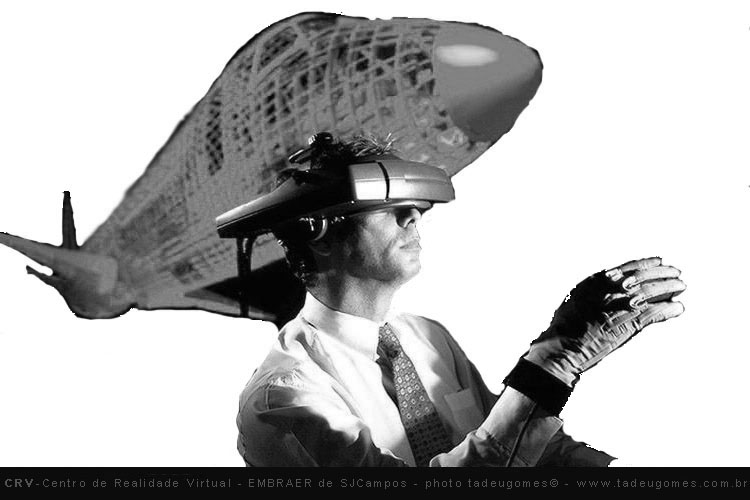
\includegraphics[scale=0.5]{images/realidade-virtual}
\caption{Aplica��o de realidade virtual}
\label{fig:realidadevirtual}
\end{figure}


\section{Realidade Aumentada}
A realidade aumentada como citado em \cite{SurveyAR} � uma t�cnica de vis�o
computacional em que valendo-se de artefatos do mundo real tem por objetivo causar sensa��o de imers�o 
do usu�rio em um ambiente aumentado por artefatos virtuais, ao contr�rio de ambientes puramente virtuais 
como � comum em aplica��es de realidade virtual.
Idealmente o mundo virtual se torna imersivo o suficiente para que o usu�rio n�o consiga distinguir o real do virtual.
Alguns autores definem AR como tendo a necessidade de utilizar-se interfaces visuais port�teis para que a 
usabilidade tenha mais coer�ncia com a proposta inicial de garantir uma experi�ncia imersiva.
As imagens s�o obtidas por c�meras e o resultado apresentado em dispositivos como projetores ou 
displays como monitores, tablets ou \emph{head-mounted display} (HMD).
Realidade aumentada pode ser realizada com ou sem marcadores para facilitar o
reconhecimento e posicionamento de entidades. No presente trabalho � utilizada a
abordagem sem marcadores para que aplica��es no cen�rios de manuten��o se torne
mais flex�vel no que tange � aplicabilidade e configura��o inicial, n�o sendo
necess�rio modificar o ambiente.A figura~\ref{diagram:pipelinera} apresenta um
pipeline b�sico de realidade aumentada de forma can�nica. O presente trabalho,
trata de aspectos at� a etapa de reconhecimento.
As etapas s�o representadas por:
\begin{itemize}
  \item \textbf{Captura:} Etapa de obten��o de imagens, feita por sensores como
  c�meras;
  \item \textbf{Prepara��o:} Etapa de prepara��o da imagem, aplicando filtros
  para a etapa de detec��o; 
  \item \textbf{Detec��o:} Etapa de detec��o de padr�es, em que s�o removido
  informa��es das imagems;
  \item \textbf{Reconhecimento:} Etapa de reconhecimento de padr�es e compara��o
  das caracter�sticas reconhecidas na etapa anterior;
  \item \textbf{Rastreio:} Etapa que garante-se que a imagem reconhecida
  continua no contexto, reconhecendo apesar de movimenta��es ou outras
  varia��es;
  \item \textbf{Apresenta�ao:} Etapa em que s�o desenhado na tela representa��es
  dos objetos reconhecidos de acordo com a aplica��o.
\end{itemize}

\begin{figure}[H]
\centering
\begin{tikzpicture}[scale=1.5 ,transform shape]

  \node[draw,rectangle] (a) {Captura};
  \node[draw,rectangle,below of=a] (b) {Prepara��o};
  \node[draw,rectangle,below of=b] (c) {Detec��o};
  \node[draw,rectangle,below of=c] (d) {Reconhecimento};
  \node[draw,rectangle,below of=d] (e) {Rastreio};
  \node[draw,rectangle,below of=e] (f) {Apresenta��o};

  % 1st pass: draw arrows
  \draw[vecArrow] (a) to (b);
  \draw[vecArrow] (b) to (c);
  \draw[vecArrow] (c) to (d);
  \draw[vecArrow] (d) to (e);
  \draw[vecArrow] (e) to (f);
    
    
  % 2nd pass: copy all from 1st pass, and replace vecArrow with innerWhite
  \draw[innerWhite] (a) to (b);
  \draw[innerWhite] (b) to (c);
  \draw[innerWhite] (c) to (d);
  \draw[innerWhite] (d) to (e);
  \draw[innerWhite] (e) to (f);

  % Note: If you have no branches, the 2nd pass is not needed

\end{tikzpicture}
  \caption{Pipeline Can�nico de Realidade Aumentada}
  \label{diagram:pipelinera}

\end{figure}




\section{Dispositivos}
 Para que a experi�ncia de imers�o seja
 completa, podem ser usados alguns dispositivos como �culos especiais, monitores
 ou projetores \cite{Devices}.

\subsection{\emph{Head-Mounted Displays}}
� um equipamento utilizado na cabe�a de forma que as duas m�os do usu�rio fiquem livres e tem por objetivo 
exibir imagens e �udio, sendo uma interface muito utilizada tanto em VR quanto
em AR.
Os HMD basicamente s�o dispositivos constitu�dos por duas telas posicionadas
frente ao olho do usu�rio.
A tecnologia pode ser empregada para exibir imagens estereosc�picas
apresentando os respectivos pontos de vista de cada olho para cada tela, o que contribui em muito na experi�ncia de imers�o.
Esses dispositivos funcionam tamb�m como entrada de dados,
porque cont�m sensores de rastreamento que medem a posi��o e orienta��o da
cabe�a, transmitindo esses dados ao computador.
Existem dois tipos de HMDs: \emph{Feed-Through} e \emph{See-Through}

\subsubsection{\emph{Feed-Through}}
S�o dispositivos que representam um sistema fechado de visualiza��o de
imagens, como mostrado na figura~\ref{fig:feedthrough}, em que o usu�rio
consegue enxergar somente o que � mostrado no \emph{display}, sendo assim, o
resultado apresentado � sempre a soma da imagem real com informa��es superpostas.

\begin{figure}[H]
\centering
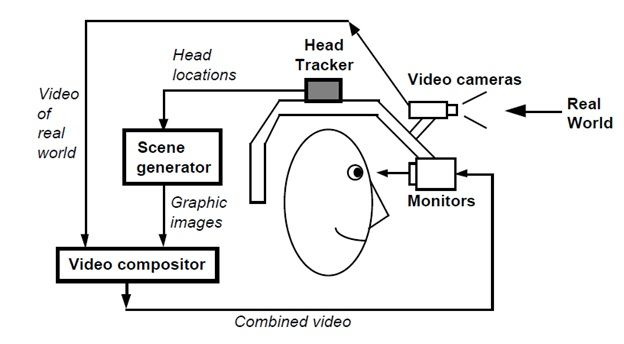
\includegraphics[scale=0.8]{images/feedthrough}
\caption{Arquitetura do \emph{Feed-Trough}. Fonte \cite{Devices}}
\label{fig:feedthrough}
\end{figure}


\subsubsection{\emph{See-Through}}
S�o dispositivos constru�dos com lentes transl�cidas em que o usu�rio enxerga o
mundo real e com algum tipo de sistema que sobrepoe na lente as informa��es
adicionais. Como mostrado na figura~\ref{fig:seethrough}:

\begin{figure}[H]
\centering
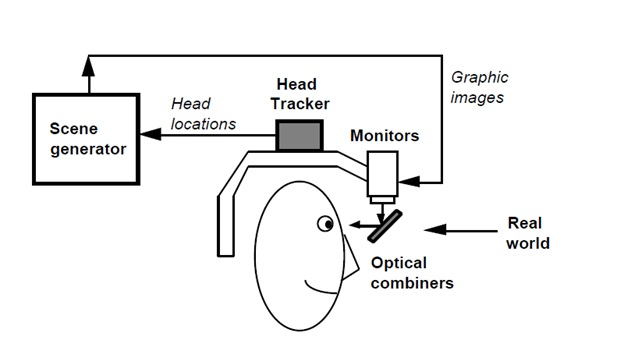
\includegraphics[scale=0.8]{images/seethrough}
\caption{Arquitetura do \emph{See-Trough}. Fonte \cite{Devices}}
\label{fig:seethrough}
\end{figure}


\subsection{Projetores}
O uso de projetores possibilita uma abordagem de realidade aumentada diferente porque pode ser
 utilizada para cobrir superf�cies largas, projetando sobre objetos como carros, pessoas, pr�dios, etc�.
Um problema dessa abordagem � que a calibra��o se faz necess�ria em situa��es
como superf�cies irregulares ou n�o paralelas ao projetor.

\subsection{Monitores}
O uso de monitores reduz bastante o custo da aplica��o apesar de ter perda de
imers�o por ser um m�todo de visualiza��o indireta, o que implica o usu�rio
ficar olhando na dire��o do monitor. Entretanto, existe a possibilidade de
compartilhar os resultados da AR com mais de uma pessoa ao mesmo tempo. Como
mostrado na figura~\ref{fig:monitores}:

\begin{figure}[H]
\centering
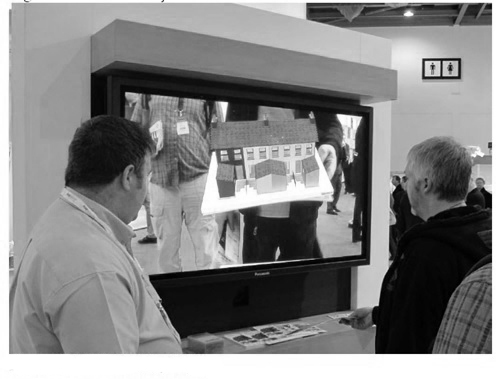
\includegraphics[scale=0.7]{images/monitores}
\caption{Realidade Aumentada com projetores. Fonte \cite{Devices}}
\label{fig:monitores}
\end{figure}

\section{Modelo de C�mera}
As c�meras s�o modeladas como c�meras de pequenos orif�cios como mostrada na
imagem~\ref{fig:camera01}.Esse modelo define a proje��o b�sica sobre a qual as
imagens 2D ser�o mapeadas.
Esse modelo � uma simplifica��o optica de uma c�mera real e � utilizado
comumente para descrever a forma��o de imagens na c�mera. O sistema de
coordenadas considerado � a conven��o da m�o direita com centro de coordenadas
de proje��o na origem e a imagem a uma dist�ncia focal f. ref[3]



\begin{figure}[h!]
\centering
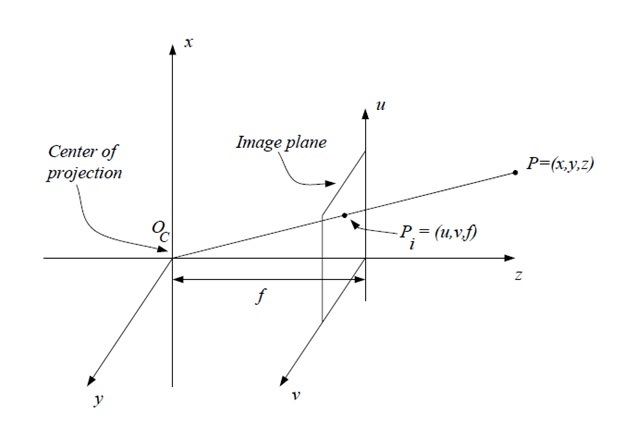
\includegraphics[scale=0.8]{images/camera01}
\caption{Camera no espa�o vetorial.}
\label{fig:camera01}
\end{figure}

\subsection{Calibra��o da C�mera}

Visto que as c�meras atuais adicionam distor��es, se faz necess�rio normalizar as
 imagens antes de utiliz�-las para que os pontos de refer�ncia n�o distor�am tanto na imagem como um todo,
  podendo sofrer efeitos de distor��o nas bordas por exemplo.
Considerando um modelo matem�tico que corrija as distor��es radiais e tangenciais. 
Para corrigir o fator radial, consideramos a seguinte transformada
\begin{figure}[h!]
\centering
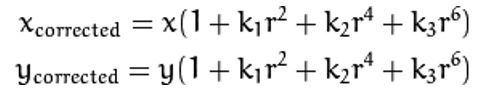
\includegraphics[scale=0.8]{images/camera_eq01}
\caption{Transforma��o de coordenadas}
\label{fig:camera_eq01}
\end{figure}


Em que (x,y) s�o a posi��o do ponto na imagem distorcida,
k1,k2 e k3 s�o constantes a serem descobertas pelo m�todo de calibra��o
r
Para corrigir a distor��o tangencial because image taking lense is not aligned perfectly parallel to the imaging plane.
 So some areas in image may look nearer than expected. It is solved as below:
 
 \begin{figure}[h!]
\centering
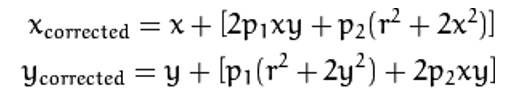
\includegraphics[scale=0.8]{images/camera_eq02}
\caption{Transforma��o de coordenadas quanto � distor��o radial}
\label{fig:camera_eq02}
\end{figure}

Para corrigirmos os dois efeitos e obtermos uma imagem calibrada temos que
resolver a matrix da imagem~\ref{fig:camera_eq03}

 
 \begin{figure}[h!]
\centering
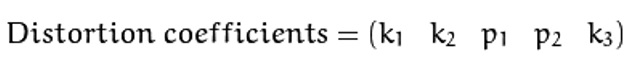
\includegraphics[scale=0.8]{images/camera_eq03}
\caption{Matriz de distor��es}
\label{fig:camera_eq03}
\end{figure}



\section{Reconhecimento}

� a etapa em que padr�es s�o identificados e comparados para posteriormente identificar objetos

 
\begin{figure}[h!]
\centering
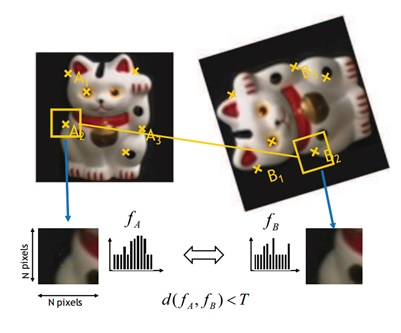
\includegraphics[scale=1.0]{images/reconhecimento}
\caption{Ilustra��o do procedimento de reconhecimento com features locais.}
\label{fig:reconhecimento}
\end{figure}

Pipeline de reconhecimento como ilustrado na imagem~\ref{fig:reconhecimento} :
\begin{itemize}
	\item Encontrar um grupo de keypoints distintos
	\item Definir uma regi�o em torno de cada keypoint 
	\item Extrair e normalizar o conte�do da regi�o
	\item Calcular um descritor para a regi�o normalizada
	\item Encontrar correspond�ncias de descritores.  
\end{itemize}


\section{Caracter�sticas Locais}
Caracter�sticas locais s�o padr�es em imagens que diferenciam padr�es de seu
vizinho imediato, sendo que as mais comuns s�o intensidade, cor e texturas.

\subsection{Caracter�sticas}
Antes de compreender como � feito o reconhecimento e registro de imagens � importante nos perguntar
 como n�s conseguimos reconhecer objetos em uma cena, como conseguimos comparar facilmente objetos em duas 
 imagens distintas. Somos treinados desde cedo a diferenciar formas geom�tricas, perceber escalas diferentes 
 ou mesmo reconhecer o mesmo objeto independente de como est� posicionado na cena buscando padr�es que 
 categorizem e diferenciem o objeto. Instintivamente conseguimos reconhecer boas caracter�sticas e localizar objetos.
Na Figura~\ref{fig:padroes} temos uma Figura de um pr�dio e seis recortes, dos quais
conseguimos facilmente reconhecer com precis�o a de letra E e F, as de letra A,B,C,D
 podemos identificar poss�veis localiza��es mas n�o podemos dizer com certeza onde est�o na Figura.

\begin{figure}[H]
\centering

\includegraphics[scale=1.0]{images/features}
\caption{Reconhecimento de padr�es. Fonte \cite{understandingfeatures}}
\label{fig:padroes}
\end{figure}
As caracter�sticas E e F s�o o que consideramos boas caracter�sticas, pois o
n�vel de certeza � bem alto.

\begin{figure}[H]
\centering
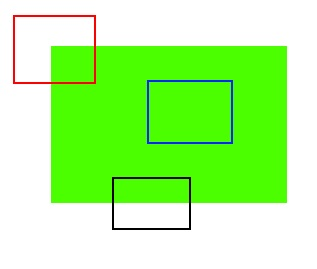
\includegraphics[scale=1.0]{images/featuresregioes}
\caption{Regi�es de reconhecimento de padr�es. Fonte
\cite{understandingfeatures}}
\label{fig:featuresregioes}
\end{figure}

A Imagem~\ref{fig:featuresregioes} ilustra tipos de caracter�sticas. A regi�o
azul n�o possibilita diferenciar onde est� na Figura, a regi�o preta pode ser confundida com qualquer uma das regi�es
 ao deslocarmos horizontalmente, a Figura vermelha nos possibilita diferenciar e reconhecer o canto da Figura verde 
 com precis�o milim�trica.
Podemos ent�o concluir que uma caracter�stica � boa para ser utilizada como par�metro de entrada
 para algoritmos de reconhecimento, quanto maior foi o n�vel de certeza da sua localiza��o, 
 o que facilita o \emph{\textbf{Feature Detection}}.
Para localizar o mesmo objeto em outra Figura � necess�rio identificarmos a regi�o onde se encontra, 
caso contr�rio no exemplo da Figura~\ref{fig:padroes} seria imposs�vel
localizar uma janela espec�fica. Tal descri��o de contexto � chamada de
\emph{\textbf{Feature Description}}. Uma vez de posse da caracter�stica e do seu
contexto � poss�vel reconhecer o objeto de fato.


\subsection{Propriedades da Caracter�stica Local ideal}
Algoritmos de reconhecimento baseam-se em compara��es de caracter�sticas
recuperadas da cena.
A recupera��o e compara��o de pontos tem um custo computacional relevante perto do tempo de execu��o 
da aplica��o, portanto selecionar o menor n�mero poss�vel de caracter�sticas aumenta o desempenho e diminui 
o tempo de resposta da aplica��o.
Garantir que  s�o selecionadas boas caracter�sticas pode ser
crucial na efic�cia do reconhecimento.
Segundo \cite{localfeaturedetector} , boas caracter�sticas devem ter as
seguintes propriedades:

\begin{itemize}
	\item \textbf{Repetibilidade}: Dadas duas imagens do mesmo objeto ou cena,
	tomadas em condi��es ou pontos de vista diferentes, uma porcentagem alta de caracter�sticas deve
	 ser reconhecida se estiverem vis�veis.
	\item \textbf{Distin��o}: Os padr�es reconhecidos t�m de ser poss�veis de serem
	distinguidos entre si para facilitar o casamento.
	\item \textbf{Localidade}: As caracter�sticas devem ser locais para reduzir a
	probabilidade de oclus�o.
	\item \textbf{Quantidade}: O n�mero de pontos detectados tem que ser o
	suficiente para que mesmo objetos pequenos tenham minimamente caracter�sticas que possam ser localizados e para que o 
	objeto possa sofrer oclus�o e ainda assim ser reconhecido.
	\item \textbf{Exatid�o}: As caracter�sticas detectadas tem que ser localizadas
	com o m�ximo de exatid�o poss�vel com respeito tanto referente � posi��o quanto
	� escala.
	\item \textbf{Efici�ncia}:De prefer�ncia  a detec��o deve ser o mais r�pido
	poss�vel.
\end{itemize}



\subsection{Detec��o de caracter�sticas}
O primeiro passo para o reconhecimento de objetos � a detec��o de caracter�sticas.Para que possa ser feita a compara��o da
 imagem referencia com a imagem sentida. A abstra��o de informa��es a ser reconhecida tem que ser suficiente para lidar 
 com escalas diferentes, rota��es entre as imagens, e pequenas distor��es.
Para que o reconhecimento seja eficiente e eficaz s�o necess�rios que uma massa de pontos m�nima seja selecionada e feita
 a correspond�ncia entre as imagens sentidas e refer�ncia.
As caracter�sticas utilizadas s�o em geral cantos, linhas, curvas, padr�es ou regi�es.
O tipo de caracter�stica selecionada � dependente do tipo de imagem provida. Imagens de cenas
 feitas a m�o geralmente s�o compostas de segmentos de retas enquanto imagens de sat�lite s�o geralmente compostas de 
 contornos e regi�es.
Quanto mais invariantes forem as caracter�sticas encontradas, mais robusto e preciso � o processo de compara��o.

\subsection{Correspond�ncia de caracter�sticas}
A fase de correspond�ncia de caracter�sticas � feita tanto selecionando caracter�sticas na imagem refer�ncia e procurando a 
correspondente na imagem sentida ou mesmo selecionando caracter�sticas nas duas imagens independentemente e procurando a 
correspond�ncia entre elas.
Quando a caracter�stica selecionada n�o for do tipo ponto, � importante para cada par de correspond�ncias, pelo menos uma 
ponto ser determinado para que seja utilizado para determinar posteriormente os par�metros de transforma��o. Por exemplo, 
se forem selecionados padr�es como tipo de caracter�stica, o centro do padr�o � considerado o ponto, se for selecionado 
uma regi�o, o centro de massa da regi�o � o ponto de apoio, se linhas forem tomadas como tipo de caracter�stica, devem 
ser tomados intersec��es como ponto de apoio e finalmente se forem selecionadas curvas, os m�ximos locais s�o considerados
 os pontos correspondentes.
 
 \section{Algoritmos de Reconhecimento}
\label{sec:algoritmos}
Existem diversos algoritmos de reconhecimento de caracter�sticas, entretanto
 nesse artigo os testes ser�o restritos aos algoritmos BRISK, FAST, FREAK, GFTT, MSER, ORB,
 STAR, SURF, SIFT.
Este cap�tulo se prop�e a dar uma vis�o geral dos algoritmos, pois o foco do
presente trabalho est� na an�lise comparativa entre os mesmos e n�o em cada um
dos algoritmos, visto exiistir implementa��es conceituadas no OpenCV, framework
utilizado.

%\subsection{BRIEF - Binary Robust Independent Elementary Features}



 \subsection{FAST}


Segundo \cite{FAST}, � um m�todo de reconhecimento baseado em detec��o de
arestas originalmente desenvolvido por Edward Rosten e Tom Drummond. A maior
promessa do m�todo � a efici�ncia computacional O m�todo considera um c�rculo de dezesseis pixels ao redor da aresta considerada p. 
O detector original \cite{FusingPoints},\cite{VideoAnotation} classifica p como
uma aresta se existem n pixels cont�guos em um c�rculo que s�o mais brilhantes do que o pixel candidato de intensidade Ip mais
 um threshold t ou mais escuros do que Ip-t

 \begin{figure}[h!]
\centering
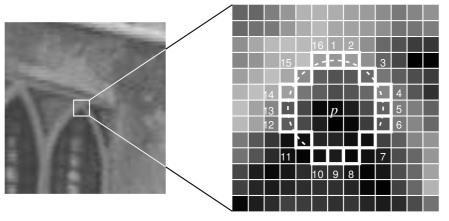
\includegraphics[scale=0.8]{images/fast01}
\caption{FAST}
\label{fig:fast01}
\end{figure}


Na imagem~\ref{fig:fast01} foi escolhido n=12. Um teste r�pido �
\begin{enumerate}
	\item Selecionar o ponto � testar primeiro as extremidades. no caso da imagem,
	escolhido o ponto p
	\item Comparar os pontos 1 e 9, e verifica-se se o ponto p tem intensidade
	com diferen�a de m�dulo t, ou seja os pontos 1 e 9 s�o mais claros ou mais escuros do que o ponto p pelo fator de t
	\item Avaliar se o ponto p continue sendo um candidato considerando os pontos 5
	e 13
	\item Analisar se p � uma aresta, sendo pelo menos 3 desses pontos devem ser
	mais brilhantes ou mais escuros do que p ent�o o teste pode ser feito nos demais pontos.
\end{enumerate}


 \subsection{BRISK - Binary Robust Invariant Scalable Keypoints}

Como descrito em \cite{BRISK}, ao contr�rio dos descritores vetoriais, como SURF
e SIFT, BRISK utiliza descritores no espa�o bin�rio o que para dispositivos com restri��o de recursos e poder computacional como dispositivos mobiles pode ser interessante.
Baseado no detector da t�cnica FAST, o processo consiste de tr�s partes.

\textbf{Amostragem de padr�es}

Retirando um padr�o de amostras ao redor do keypoint referentes a pontos espalhados em circulos conc�ntricos, que s�o usados para determinar se o ponto deve ou n�o ser selecionado como em um detector FAST.
As amostras s�o separadas em pares de dois subsets, curta dist�ncia e longa dist�ncia.

\textbf{Compensa��o de Orienta��o}
%REFAZER

Para atingir invari�ncia a rota��o, a dire��o de cada keypoint � determinada
tomando a soma dos gradientes locais calculados entre pares de longa dist�ncia e
os pares de curta dist�ncia s�o rotacionados baseados na orienta��o obtida.

\textbf{Compara��o de pares de amostragem}

 \begin{figure}[H]
\centering
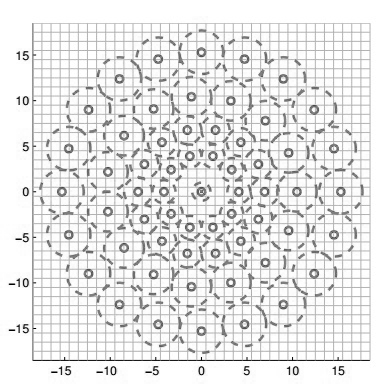
\includegraphics[scale=0.8]{images/brisk-descriptor}
\caption{Padr�o de amostras no BRISK}
\label{fig:briskdescriptor}
\end{figure}


Como mostrado na figura~\ref{fig:briskdescriptor}, BRISK possui um descritor
bin�rio de 512 bits que calcula a m�dia ponderada utilizando uma Gaussiana sobre um padr�o de pontos mais pr�ximos do ponto selecionado como mostrado na imagem~\ref{fig:briskdescriptor} no ponto (0,0). Ao longo do padr�o descrito, s�o aplicadas suaviza��es Gaussianas sendo que os c�rculos vermelhos representam o tamanho do desvio padr�o do filtro Gaussiano aplicado a cada ponto.
� baseado em compara��es entre pares de janelas de Gaussianas, resultando em 1 ou 0, dependendo de qual janela no par for maior.
Os pares ent�o s�o pr� selecionado no BRISK, criando descritores bin�rios que s�o posteriormente utilizados para casamento de padr�o, utilizando dist�ncias Hamming ao inv�s de Euclidianas.





 \subsection{FREAK - Fast Retina Keypoint}

FREAK � um descritor bin�rio, composto por tr�s etapas:

\textbf{Amostragem de padr�o}

FREAK prop�e uma abordagem biol�gica para o reconhecimento de caracter�sticas, emulando o funcionamento da retina para amostragem de padr�o, como demonstrado na imagem \ref{fig:freak-sampler} que � um padr�o circular com a diferen�a de ter maior densidade de pontos pr�ximo do centro. A densidade de pontos decresce exponencialmente.

\begin{figure}[H]
\centering
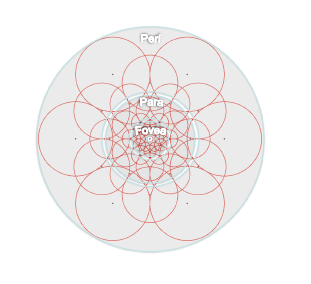
\includegraphics[scale=1.0]{images/freak-sampler}
\caption{Padr�o de amostradem do descritor FREAK}
\label{fig:freak-sampler}
\end{figure}


Cada amostra � suavizada com um kernel Gaussiano em que o raio do circulo ilustra o tamanho do desvio padr�o do kernel.
Como pode ser observado na figura~\ref{fig:freak-retina} o padr�o de amostragem corresponde com a distribui��o de receeptores na retina.

\begin{figure}[H]
\centering
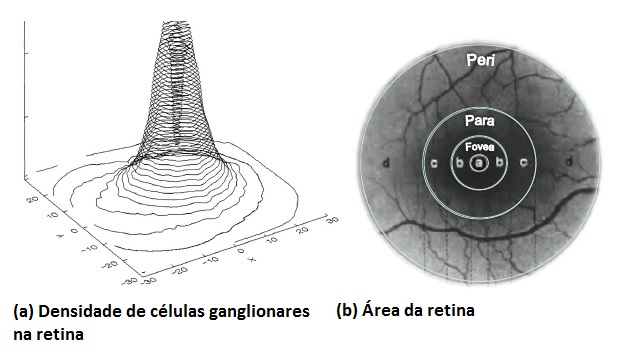
\includegraphics[scale=1.0]{images/freak-retina}
\caption{Distribui��o de receptores na retina}
\label{fig:freak-retina}
\end{figure}


\textbf{Compensa��o de Orienta��o}

Para estimar a rota��o dos keypoints, s�o somados os gradientes locais assim como no BRISK, entretanto ao inv�s de considerar os pontos de longa dist�ncia, s�o considerados 45 pontos como mostrado na figura~\ref{fig:freak-rotation}


\begin{figure}[H]
\centering
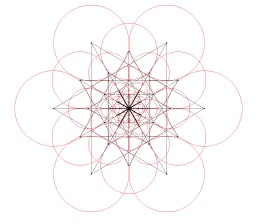
\includegraphics[scale=1.0]{images/freak-rotation}
\caption{Pares selecionados para calcular a orienta��o}
\label{fig:freak-rotation}
\end{figure}

Apesar de ter menos precis�o para recuperar informa��es de reota��o, como o n�mero de pontos � bem menor do que BRISK a quantidade de mem�ria armazenada � em geral mais do que 5 vezes menor.



\textbf{Compara��o de pares de amostragem}

Os pares de pontos s�o selecionados considerando a densidade maior no centro, como podemos observar na figura~\ref{fig:freak-retina} (a). Os pares come�am a ser comparados pelas extremidades e para dentro do centro, dessa forma otimizamos o reconhecimento pois com menos pontos podemos descartar casos em que a dist�ncia estiverem maiores do que um threshold, caso contr�rio prosseguimos para os outros 128 bits do descritor.



 \subsection{GFTT}
\label{sec:gftt}
 \subsection{MSER - \emph{Maximal Stable Extremal Regions}}

O detector MSER � composto por regi�es de todos os pixels conectados
considerando um \emph{threshold}. Em outras palavras, as regi�es selecionadas
s�o padr�es que n�o mudam e que a binariza��o local � est�vel ao longo de uma
faixa de \emph{thresholds}. Podemos fazer uma
analogia com o processo de forma��o de po�as de �gua para compreendermos como
s�o formadas as regi�es MSER, que s�o descritas em imagens em tons de cinza
representados pela fun��o $I: \Omega \rightarrow [0\ldots255] $ em que $\Omega =
[1 \ldots W]\times[1 \ldots H] $. O m�todo garante a localiza��o de objetos que
est�o mais pr�ximos de nossa realidade como pode ser observada na
Figura~\ref{fig:mserregion} \cite{MSER}.

 \begin{figure}[H]
\centering
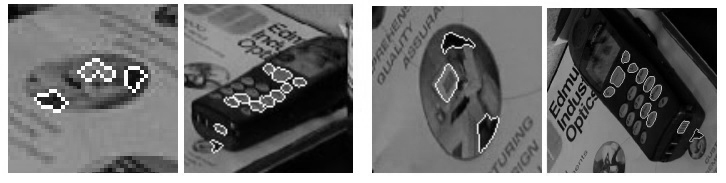
\includegraphics[scale=0.5]{images/mserregion}
\caption{Regi�es MSER. Fonte \cite{MSER}}
\label{fig:mserregion}
\end{figure}

Selecionado um \emph{threshold} de intensidades, a Figura � dividida em dois
grupos, P(pretos) e B(brancos). � observada que a quantidade de regi�es varia
dependendo do \emph{threshold} aplicado, de 0 a 255.
A �rea de cada componente conectado � ent�o armazenada como uma fun��o. Dentre
as regi�es, as mais est�veis s�o selecionadas analisando as fun��es para as quais
cada regi�o em potencial mantem seu estado com a mesma fun��o independente da
varia��o de \emph{threshold}. As regi�es ``m�ximamente est�veis'' s�o chamadas
regi�es MSER, que mudaram apenas em tamanho variando-se pelo menos alguns n�veis
de \emph{threshold}.




 \subsection{ORB - Oriented Fast and Rotated Brief}
\label{sec:orb}

%REFAZER
Como citado em \cite{ORB}, � uma combina��o de FAST e BRIEF.
 Para extrair \emph{keypoints}, modifica o detector do FAST construindo uma 
 piramide de escalas das imagems. Em cada escala \emph{keypoints} s�o
 detectados e a dist�ncia de Harris aplicada para selecion�-los, sendo somente
 os N melhores pontos selecionados de acordo com um \emph{threshold}.
Para obter invari�ncia � rota��o, momentos de primeira ordem s�o utilizados
 para calcular a orienta��o local atrav�s de um centr�ide que referencia a
  m�dia da magnitude dos pixels em um trecho local.
Posteriormente s�o calculados os descritores BRIEF nos trechos rotacionados
 e armazenadas as informa��es em um descritor ORB.




 \subsection{SIFT - Scale-Invariant Feature Transform}

M�todo baseado em detec��o de arestas que tem como proposta garantir a
invariancia a varia��o de escala. Um problema que nos m�todos de reconhecimento
de arestas se n�o tratado pode causar diminui��o na robustes do algoritmo. 
A figura~\ref{fig:sift01} ilustra bem o efeito que a mudan�a de escala pode
fazer.

\begin{figure}[h!]
\centering
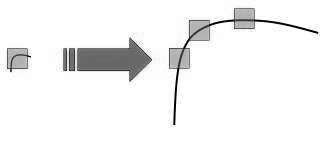
\includegraphics[scale=1.0]{images/SIFT01}
\caption{SIFT}
\label{fig:sift01}
\end{figure}

Em 2004, D.Lowe, descreveu o algoritmo Scale Invariant Feature Tranform no seu paper Distinctive Image
 Features from Scale-Invariant Keypoints[15] como extrair keypoints e computar os descritores.
8.10.2.1. Scale-space Extrema Detection
Observando a imagem~\ref{fig:sift01} � poss�vel notar que n�o podemos utilizar a
mesma janela de inspe��o independente da escala do objeto, para objetos maiores
temos que utilizar janelas maiores. Nesse contexto, o filtro scale-space �
utilizado e s�o calculados Laplacianos de Gaucianos com diversos valores de
$\sigma$.
  Os LoG funcionam como blob detectors que detectam
 blobs em v�rias escalas com a varia��o de $\sigma$.

Utilizar Laplacianos de Gaucianos � uma abordagem custosa computacionalmente,
como uma forma de aproxima��o s�o utilizados diferen�as de Gaucianas.


\begin{figure}[h!]
\centering
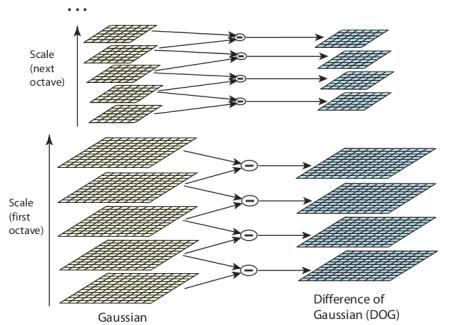
\includegraphics[scale=1.0]{images/DoG}
\caption{Difference of Gaussian}
\label{fig:dog01}
\end{figure}

Uma vez que as diferen�as de gaucianas s�o calculadas, � necess�rio procurar por
m�ximos entre espa�o e escalas diferentes. Por exemplo como mostrado na
figure~\ref{fig:dog02}, um pixel na imagem � comparado com seus 8 vizinhos e com
n�veis de escala pr�ximos e anteriores.
O que representa que o keypoint encontrado � melhor representado naquela escala.

\begin{figure}[h!]
\centering
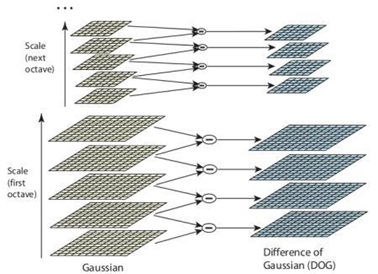
\includegraphics[scale=1.0]{images/DoG_escala}
\caption{Difference of Gaussian}
\label{fig:dog02}
\end{figure}



\subsubsection{Keypoint Localization}
Uma vez que keypoints potenciais s�o localizados � importante selecionar pontos de interesse com contraste alto.
A localiza��o dos pontos � refinada utilizando uma expans�o de Taylor  e se as intensidades dos m�ximos forem 
menores do que um threshold s�o rejeitados.
Uma caracter�stica do DoG � a alta resposta a arestas gerando falsos positivos. Portanto � necess�rio eliminar 
algumas arestas identificadas erroneamente.
\subsubsection{Orientation Assignment}
TODO
\subsubsection{Keypoint Descriptor}
TODO
\subsubsection{Keypoint Matching}
O casamento entre dois pontos � feito identificando pontos pr�ximos. Entretando em algumas citua��es existem
 pontos muito pr�ximos que podem ser causados por ruidos na detec��o de pontos de interesse, nesse caso � calculada
  uma raz�o de dist�ncia entre o ponto de interesse com o mais pr�ximo, e com o segundo mais pr�ximo, se a raz�o for
   maior do que 80 s�o rejeitados. Tal abordagem elimina cerca de 90 de falsos positivos e 5 de pontos corretos.




 \subsection{SURF - Speeded Up Robust Feature}

Segundo \cite{SURF} em compara��o com o algoritmo SIFT que aproxima Laplacianas
de Gaucinas por Diferencas de Gaucianas(DoG), SURF aproxima LoG de Box-type Filter e n�o �
utilizado nenhum tipo de suaviza��o entre escalas , o que garante mais agilidade
nos resultados porque a convolu��o com box filters s�o muito mais r�pidos com o uso de
 integral images e pode ser paralelizado

\begin{figure}[h!]
\centering
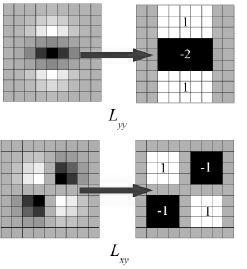
\includegraphics[scale=1.0]{images/SURF01}
\caption{Box Filtering}
\label{fig:surf01}
\end{figure}

Em geral SURF se apresenta cinco vezes mais r�pido do que DoG.
 \subsection{STAR}

Derivado de CenSurR(\emph{Center Surround Extrema}), STAR\cite{STAR}, assim como
SURF citado na Se��o~\ref{sec:surf} � baseado em \emph{box filters}. Entretanto,
enquanto DoB n�o � invariante � rota��o, � introduzido o filtro
\emph{center surroung} que s�o bi-level. A Figura~\ref{fig:bilevelfilter} mostra
o padr�o do filtro bi-level em v�rios n�veis, sendo o quanto mais circular, mais
preciso, entretanto tamb�m mais dif�cil de se calcular.
 
\begin{figure}[H]
\centering
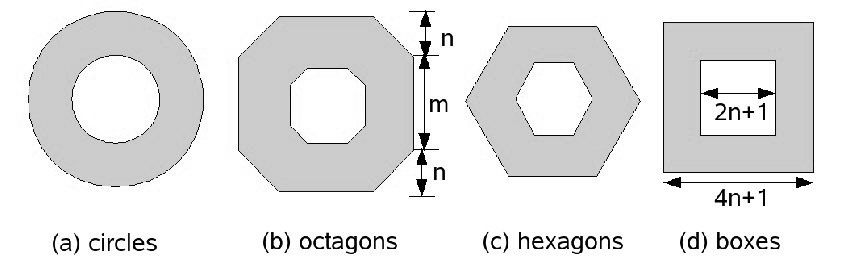
\includegraphics[scale=0.4]{images/bilevelfilter}
\caption{Filtro bi-level aplicado � formas de n lados. Fonte \cite{STAR}}
\label{fig:bilevelfilter}
\end{figure}


O detector de caracter�sticas de STAR em contrapartida � proposta do CenSurE,
usa um filtro composto de dois quadrados rotacionados. A resposta do filtro � calculada para sete escalas em cada pixel
da imagem. Em contraste com SIFT e SURF, o tamanho da amostra � constante em
cada escala e tende � resolu��o total em cada escala.
Um passo de p�s processamento � realizado para suprimir os n�o m�ximos e as
linhas.
Caracter�sticas que est�o ao longo de linhas s�o detectador devido � matriz de
gradientes, como apresentado na equa��o~\ref{eq:gftt}.





\section{Cad�ncia}
� a medida do n�mero de quadros individuais que um determinado dispositivo �ptico ou eletr�nico processa e exibe
 por unidade de tempo. Em geral a cad�ncia � medida em fps.
Em cinema, a cad�ncia de proje��o padr�o desde 1929 foi fixada em 24fps, sendo
no per�odo do cinema mudo a maioria dos filmes eram rodados com cad�ncia entre 16 e 20fps.
Em v�deo, os principais sistemas lidam com cad�ncia entre 25fps(PAL) e 30fps(NTSC).
As aplica��es devem ter cad�ncia toler�vel dependendo de seu uso, segundo
\cite{Tang93whydo} para aplica��es interativas o m�nimo toler�vel � de 5fps enquanto para aplica��es
 de anima��es fluidas de 30fps.
Sendo a cad�ncia a freq��ncia entre frames, deve ser contabilizado o tempo de
gera��o de informa��es e o tempo de dispor a informa��o no dispositivo �ptico.
O tempo de cada frame � calculado  o inverso do n�mero de fps.
%como mostrado na
%equa��o~\ref{eq:fps}
%\begin{equation}
%t_{frame} =  \frac{1}{fps}
%\label{eq:fps}
%\end{equation}
No caso de cad�ncia m�nima de 5fps, temos quadros com tempo menor que 200ms,
portanto as an�lises devem ser balizadas a tempos menores.







